\section{LOGICAL MODEL STRUCTURE}\label{sec:dataware}

The logical model of the data warehouse is a snowflake schema as shown in Figure \ref{fig:datawarehouse}. It consists of a total amount of 8 different tables, 3 of those being fact tables. Trivial dimensions like Date and Time will not be described in depth. The color encoding is as following; Purple entities are solely on the clients side, the red entities are on both the clients side and the insurance companys side. The green entity is implemented on the client side, and has special situational relation to the insurance company, which will be described in depth in the next paragraph.

\begin{figure*}[tb]
\centering
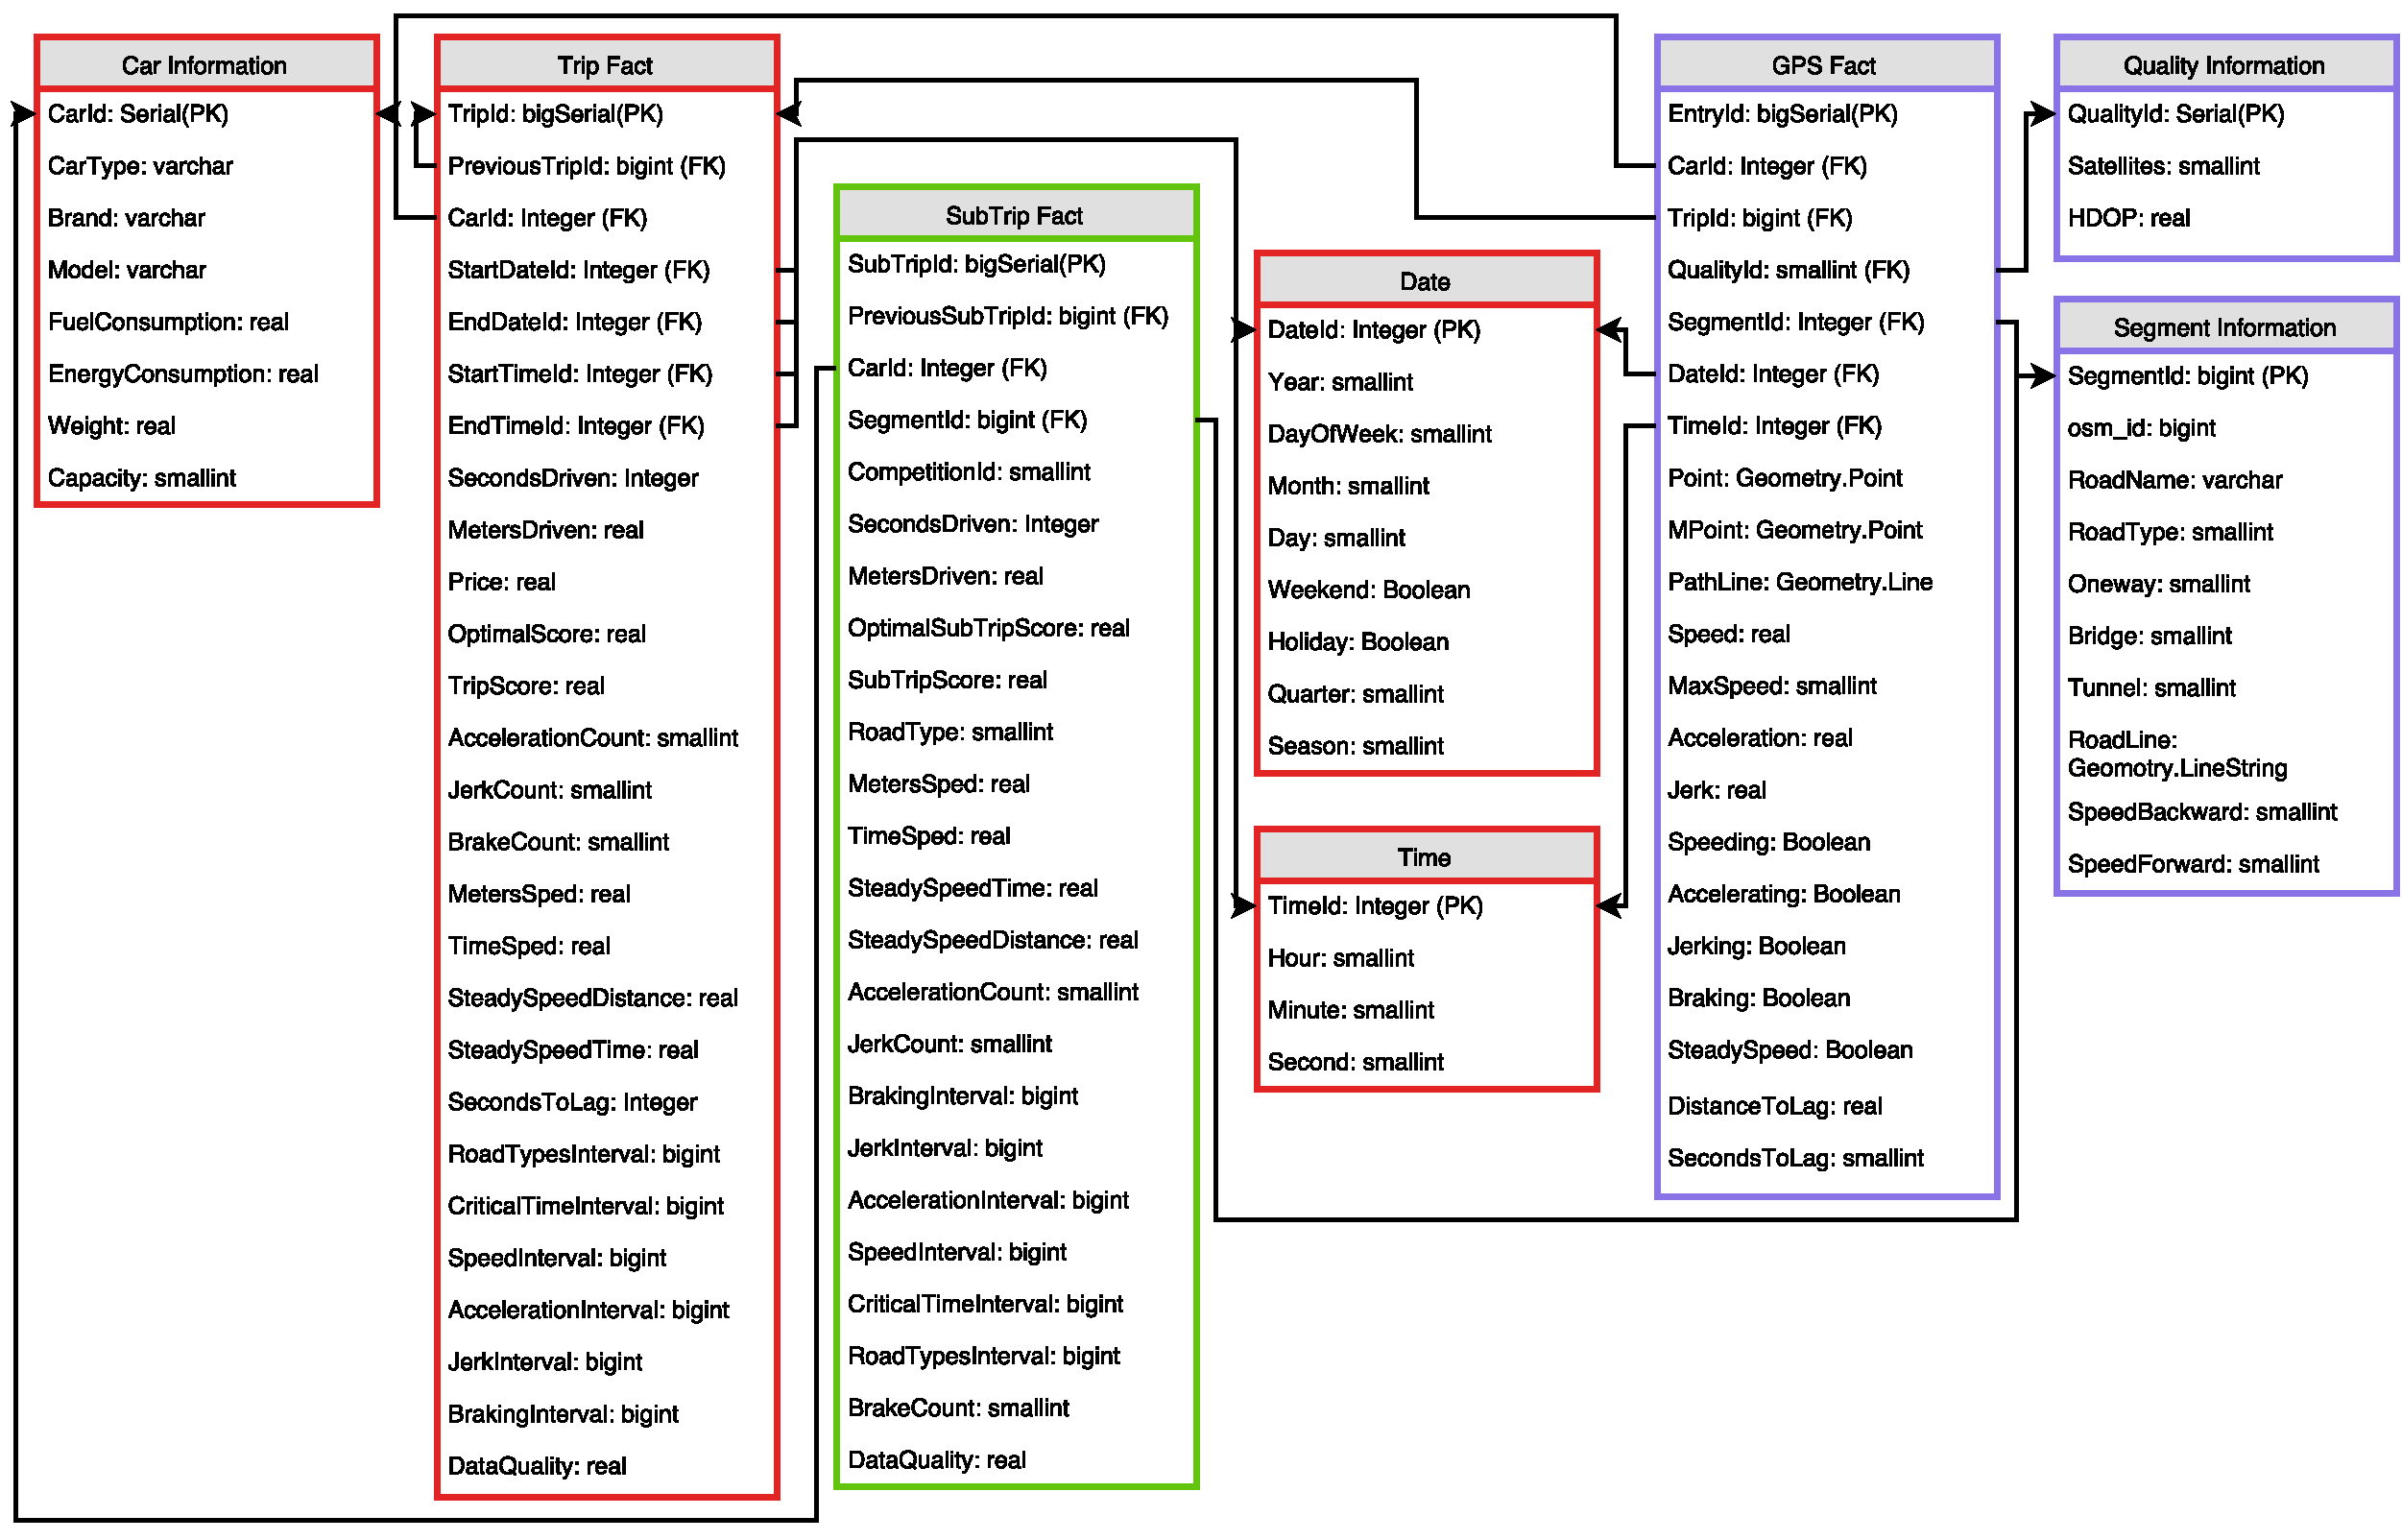
\includegraphics[width=0.9\textwidth]{Pictures/ERDiagram}
\caption{Logical Model of the Data Warehouse}
\label{fig:datawarehouse}
\end{figure*}

\subsection{Fact Tables}

Amongst the fact tables there is a certain hierarchy, the GPS fact table is the main fact table where each entry is logged through the logging device. Certain values are calculated on the logged entry, and added to the database. After the journey has ended, a tripfact is then calculated given the gpsfacts. Subtripfacts are calculated from the gpsfacts associated with each segmentid in the journey. The interaction will be further described in \nameref{sec:ETL}.

\textbf{GPS Fact} is the center of the entire data warehouse. Each entry represents a singular GPS point of a car, with the actual timestamps. The table references all of the support tables, as well as a reference to a single tripfact. A GPS fact contains spatial attributes in \textit{Point},\textit{MPoint} and \textit{PathLine}, being GPS coordinates, map-matched GPS coordinates and a line to the previous GPS coordinate respectively. A gpsfact contains a lot of Booleans, namely \textit{Speeding}, \textit{Accelerating}, \textit{Jerking}, \textit{Braking} and \textit{SteadySpeed}, which is primarily added for querying as the actual value exists in different attributes. The actual values of the attributes are all calculated in relation to the previous points e.g. acceleration is the change in speed between now and previous point divided with the distance between them.

\textbf{Trip Fact} entries represents an actual car trip through a sample of GPS coordinates. They contain a start-time and an end-time represented by 4 foreign keys to the Date and Time dimensions. A tripfact has a lot of attributes which is simply an addition from the sample of gpsfacts, namely \textit{MetersDriven}, \textit{SecondsDriven} and all of the count attributes. Each trip fact has a \textit{TripScore} and \textit{OptimalScore} which is the calculated score dependant on the insurance policy used, as well as the optimal score for the given trip, this will be described later in \ref{sec:trip}. A contribution of this article is the decision create intervals in the form of a bigInt, to represent to which degree the actual delinquency is. To explain this further, here is a clean example in Table \ref{tab:intervalexampe} with Acceleration; 

\begin{table}[h]
\centering
\begin{tabular}{cc | cc}
\multicolumn{2}{c}{\textbf{Policies}} & \multicolumn{2}{c}{\textbf{Logged Info}} \\\hline
\textbf{Intervals ($m/s^{2}$)}     & \textbf{Weights}     & \textbf{Amount}     & \textbf{Percentage}     \\\hline
{[}3, 4 {[}              & 1.05              &   32            & 40              \\
{[}4, 4.5 {[}            & 1.10              &   16            & 20              \\
{[}4.5, 5 {[}            & 1.15              &   8             & 10              \\
{[}5, 5.5 {[}            & 1.25              &   4             & 5              \\
{[}5.5, 6 {[}            & 1.35              &   8             & 10              \\
{[}6, 6.5 {[}            & 1.45              &   4             & 5              \\
{[}6.5, 7 {[}            & 1.55              &   8             & 10              \\
{[}7, $\infty$ {]}       & 1.80              &   0             & 0              \\\hline
\end{tabular}
\caption{An example of Acceleration Interval}
\label{tab:intervalexampe}
\end{table}

All of the accelerations for the trip are divided into different intervals depending of their severity. The intervals and weight is determined by some policy presented by the insurance company, meaning you can have different policies throughout the system. The policy is represented by the 2nd and 3rd digit in the bigInt. As the total amount of delinquencies can extend 100, and there is only 2 digits representing each number, the percentage is used instead. If one of the intervals contains 100\% of the delinquencies the 1st digit of the bigInt is set to 1. So this particular example would result in the following bigInt;

$$
0\ 01\ 32\ 16\ 08\ 04\ 08\ 04\ 08\ 00 \eqno{(1)}
$$
given the policy's id is 1.

\textbf{SubTrip Fact} is a special fact table in the sense that it does not have any direct impact on the insurance. It is created with gamification in mind, making it possible to compare different clients to each other on certain segments. Direct comparison between full tripfacts are hard because the routes are quite unique. Aside from only covering a certain segment, the SubTrip Fact table is very similar to the Trip Fact. One of the more noticable differences however are the fact that a subtripfact has a \textit{competitionId}, which makes it possible for the insurance company to create competitions on certain segments.


\subsection{Information Tables}

\textbf{Car Information} is a support table holding valid information about the users car. The data is valuable to the insurance company, if not for actual insurance calculations, then for statistical use. The data is of a relation 1 to many tripfacts, subtripfacts or gpsfacts, meaning each of these must have a link to an entry in Car Information. This is important due to the insurance policy is per car rather than per person.

\textbf{Quality Information} is a support table which determines the quality of the given gpsfact. The table contains information on the Horizontal-Dilution-of-Position(HDOP) and the amount of satellites covering the car. Whenever the algorithm encounters a new unseen combination of the two, it creates an entry in the database. Entries are mapped 1 to many gpsfacts because of this, but  the amount of duplicated information is reduced.

\textbf{Segment Information} is the last support table and it has the entire road network of Denmark from openstreetmap. The osm\_id is kept to make it possible for cooperation and better integration in the future. Segment Information is related 1 to many to both subtripfacts and gpsfacts.